\section{Results}
\label{s:results}

Here, we show some of our reconstructions as well as illustrate the implementation of our immediate steps, such as the SIFT matching points and Zhang's method. We used a Panasonic Lumix DMC-ZS5 camera to take pictures.

\subsection{Camera Calibration}
As stated above, we use Zhang's method to calibrate our camera. We use a sheet of paper with six 2" by 2" black boxes. Some pictures of the different angles used for the calibration are shown in Figure~\ref{calib_pics}. 

\begin{figure}[H]
\begin{center}
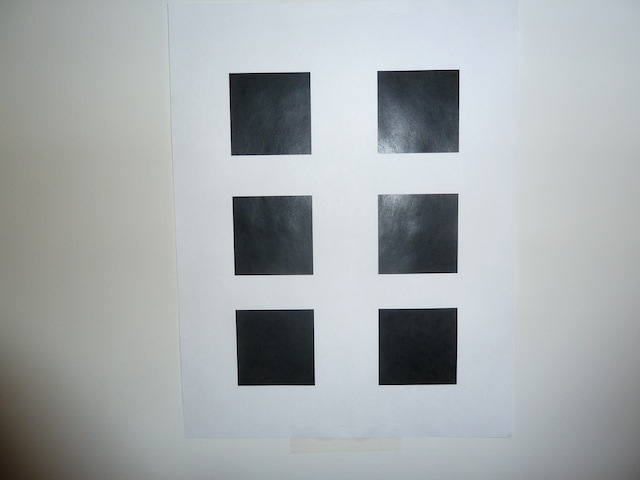
\includegraphics[width=0.45\linewidth]{figures/calib1.jpg}
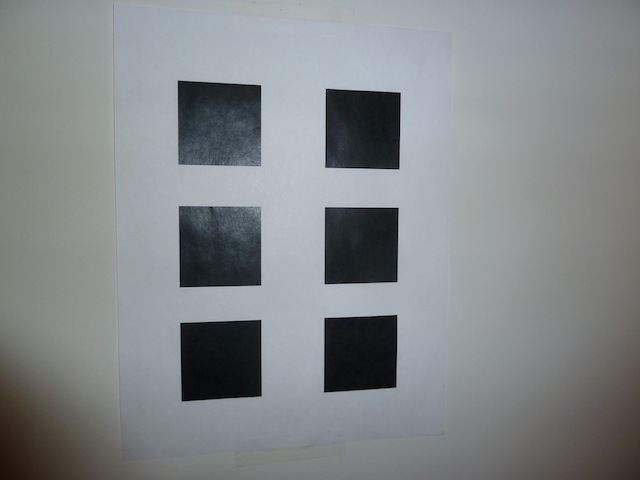
\includegraphics[width=0.45\linewidth]{figures/calib2.jpg}
\end{center}
\caption{Different calibration angles for Zhang's method}
\label{calib_pics}
\end{figure}

We used multiple views and took the average over different permutations. We found the following intrinsic parameter matrix $K$ for this camera:
\begin{equation*}
K =
  \left[ {\begin{array}{ccc}
   360.506 & -38.7974 & 128.692  \\
  0 & 470.953 & 162.864 \\
   0 & 0 & 1 \\
  \end{array} } \right]
\end{equation*}

\subsection{Reconstruction of Zhang's images}
We first reconstructed the images provided by Zhang~\cite{Calibration} because we were provided with the pictures and internal parameters. 